%==============================================================================
% Sjabloon poster bachproef
%==============================================================================
% Gebaseerd op document class `a0poster' door Gerlinde Kettl en Matthias Weiser
% Aangepast voor gebruik aan HOGENT door Jens Buysse en Bert Van Vreckem

\documentclass[a0,portrait]{hogent-poster}
\usepackage{parskip}

% Info over de opleiding
\course{Bachelorproef}
\studyprogramme{toegepaste informatica}
\academicyear{\advance\year by -1 \the\year--\advance\year by 1 \the\year}
\institution{Hogeschool Gent, Valentin Vaerwyckweg 1, 9000 Gent}

% Info over de bachelorproef
\title{De identiteit van een Linux-systeem:\\ Onderzoek en Proof of Concept.}
\author{Van Assche Anton}
\email{anton.vanassche@student.hogent.be}
\supervisor{Dhr. T. Clauwaert}
\cosupervisor{Dhr. B. Deferme (Open-Future)}

% Indien ingevuld, wordt deze informatie toegevoegd aan het einde van de
% abstract. Zet in commentaar als je dit niet wilt.
\specialisation{Systeem- en Netwerkbeheer}
\keywords{Cybersecurity, Automatisatie, Linux, Infrastructure as Code, Network and Information Security 2}
\projectrepo{https://github.com/AntonVanAssche/hogent-bachelorproef}

\begin{document}

\maketitle

\begin{abstract}
Cybersecurity en de automatisering van systemen zijn cruciaal in de IT-wereld.
Met de nieuwe NIS2-richtlijn, die bedrijven verplicht om hun systemen te beschermen tegen cyberaanvallen, is de noodzaak voor geavanceerde beveiligingsmaatregelen groter dan ooit.
Een van de eisen van deze richtlijn is het in kaart brengen van alle kritieke systemen binnen een organisatie.

Infrastructure as Code (IaC) biedt een potenti\"ele oplossing door de infrastructuur van een bedrijf in code te beschrijven, wat een overzicht van alle gebruikte systemen geeft.
Toch vinden veel KMO's het moeilijk om naar een IaC-omgeving over te stappen vanwege een gebrek aan kennis, tijd en budget.

Deze bachelorproef onderzoekt tools die de overgang naar een IaC-omgeving kunnen vergemakkelijken door het opstellen van een configuratie-inventaris.
Er wordt gekeken naar bestaande tools en hun eigenschappen, met een focus op Linux-systemen.
Een Proof of Concept zal worden ontwikkeld in de vorm van een Bash-script dat basisinformatie van Linux-systemen verzamelt en omzet in overzichtelijke bestanden.
Dit script zal worden getest op vijf verschillende Debian-servers met verschillende rollen.

Tools zoals Nmap en LinPEAS-ng zullen worden gebruikt om de configuratie van Linux-systemen te ontdekken.
Nmap richt zich op netwerkconfiguraties, terwijl LinPEAS-ng dieper inzicht biedt in de systeemconfiguratie en potenti\"ele beveiligingsrisico's identificeert.
Het script biedt een basis waarop beheerders verder kunnen bouwen, met de mogelijkheid om extra functionaliteiten toe te voegen en beperkingen aan te pakken die tijdens de ontwikkeling zijn ge\"identificeerd.

\end{abstract}

\begin{multicols}{2} % This is how many columns your poster will be broken into, a portrait poster is generally split into 2 columns

\section{Introductie}

In het begin van 2023, op 6 januari, werd de NIS-richtlijn (\textbf{Network and Information Security}) opgevolgd door zijn nieuwe versie, \textbf{NIS2}.
Deze update bracht verschillende nieuwe voorschriften met zich mee op het gebied van cyberbeveiliging en breidde het aantal sectoren dat aan deze richtlijnen moet voldoen aanzienlijk uit.

De lidstaten van de Europese Unie hebben tot oktober 2024 de tijd om deze nieuwe richtlijnen in hun nationale wetgeving te implementeren.
Dit geeft bedrijven een beperkte periode om hun processen aan te passen aan deze nieuwe wetgeving, wat vooral voor \textbf{kleine en middelgrote ondernemingen} (KMO's) een uitdaging kan zijn, gezien hun vaak beperkte middelen.

Een van de essenti\"ele vereisten van deze richtlijnen is dat bedrijven verplicht zijn om een ``\textbf{inventory of assets}'' op te stellen voor alle systemen en operaties die ze gebruiken.
Deze bachelorproef richt zich specifiek op het bieden van een oplossing voor KMO's binnen sectoren die nu moeten voldoen aan deze richtlijnen, door middel van het inventariseren van de configuratie van Linux-systemen.

Het doel is om een Bash-script te ontwikkelen dat basisinformatie van \textbf{Linux}-systemen verzamelt en omzet in overzichtelijke bestanden.
Hierdoor kunnen bedrijven op een eenvoudige manier configuraties verzamelen en vervolgens overstappen naar een \textbf{Infrastructure as Code} (IaC) omgeving.

\section{Doelstellingen}

Het doel van deze bachelorproef is om een \textbf{Proof of Concept} te ontwikkelen die KMO's helpt bij het \textbf{inventariseren} van hun \textbf{Linux-systemen} en hun \textbf{configuratie}, met behulp van een Bash-script.
Het script zal rekening moeten houden met de bevindingen uit de \textbf{risicoanalyse}, en voorgaande hoofdstukken van deze bachelorproef.

Ook zal er een kritische evaluatie worden gemaakt van de Proof of Concept, waarbij de effectiviteit en volledigheid van de inventarisatie wordt beoordeeld.

\section{Risicoanalyse}

Het doel van de risicoanalyse is om de cruciale \textbf{configuratie-eigenschappen} van Linux-systemen te \textbf{identificeren} die essentieel zijn \textbf{voor het opstellen van een inventaris}.
Hierbij wordt onderzocht wat de identiteit van een Linux-systeem bepaalt, evenals de bijbehorende beveiligingsaspecten.
De verkregen inzichten zullen dienen als basis voor de ontwikkeling van de Proof of Concept.

\section{Proof of Concept}

Tijdens de Proof of Concept wordt een \textbf{Bash-script} ontwikkeld dat basisinformatie van Linux-systemen verzamelt en omzet in overzichtelijke bestanden.
Dit script wordt vervolgens getest op een omgeving bestaande uit zes \textbf{Debian-servers} met verschillende rollen, waarvan \textbf{vijf gebruikt} zullen worden \textbf{om het script te testen} en \'e\'en om de initi\"ele configuratie vast te leggen.
De gekozen rollen dekken een breed scala aan configuraties en bieden een representatief beeld van een productieomgeving.

\begin{center}
  \begin{tabular}{ c c }
    \hline
        Servernaam & Rol \\ [0.5ex]
    \hline
    control & Ansible-controller \\
    srv1    & DNS-server \\
    srv2    & Webserver \\
    srv3    & Database-server \\
    srv4    & Monitoring-server \\
    srv5    & Fileserver \\
  \end{tabular}
\end{center}
\captionof{table}{Overzicht van de verschillende servers en hun rollen.}

\begin{center}
  \captionsetup{type=figure}
  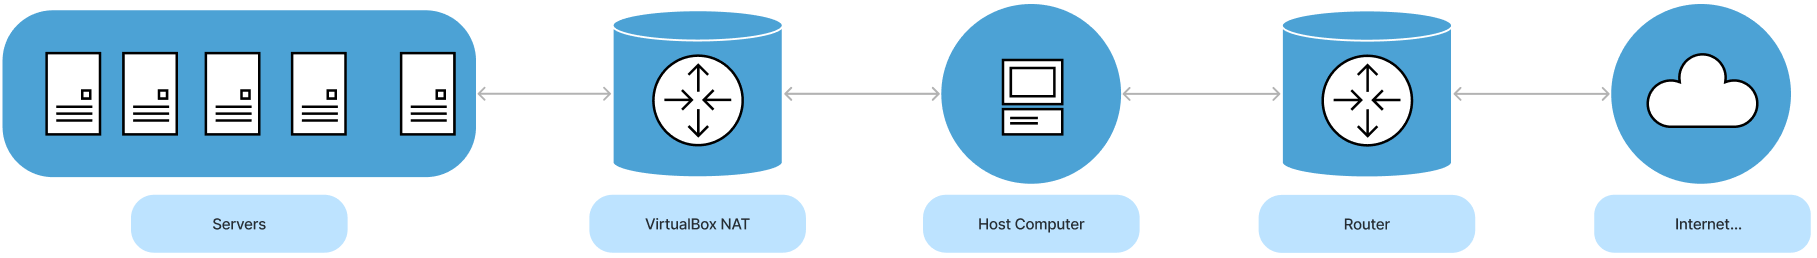
\includegraphics[width=1.0\linewidth]{env}
  \captionof{figure}{De opstellling van de testomgeving.}
\end{center}

\section{Conclusies}

\begin{enumerate}
  \item \textbf{Nmap} en \textbf{LinPEAS-ng} zijn \textbf{geschikte tools} om de configuratie van Linux-systemen te ontdekken.
    \begin{itemize}
      \item \textbf{Nmap} richt zich op \textbf{netwerkconfiguraties}.
      \item \textbf{LinPEAS-ng} biedt dieper inzicht in de systeemconfiguratie en \textbf{identificeert potenti\"ele beveiligingsrisico's}.
    \end{itemize}
  \item De \textbf{risicoanalyse} heeft de \textbf{belangrijkste configuratie-eigenschappen} van Linux-systemen \textbf{ge\"identificeerd} die essentieel zijn voor een inventaris.
  \item Het \textbf{script biedt} een \textbf{basis} waarop beheerders verder kunnen bouwen.
  \item Verdere verbeteringen en uitbreidingen van het script zijn nodig voor een robuuste inventarisatie.
\end{enumerate}

\section{Toekomstig onderzoek}

\begin{enumerate}
  \item Uitbreiden van compatibiliteit met andere Linux distributies.
  \item Functionaliteiten uitbreiden naar cloudomgevingen doormiddel van API-calls.
  \item Ondersteuning toevoegen voor AppArmor- en SELinux-configuratie.
  \item Voorzien van een mechanisme om verbinding te maken met de servers en het vervolgens het script uit te voeren.
  \item Integreren van een grondigere analyse van de CIS Benchmarks.
\end{enumerate}

\end{multicols}
\end{document}
